\documentclass[twoside,senior]{BYUPhys}
% The BYUPhys class is for producing theses and dissertations
% in the BYU department of physics and astronomy.  You can supply
% the following optional arguments in the square brackets to
% specify the thesis type:
%
%   senior  : Produces the senior thesis preliminary pages (default)
%   honors  : Produces the honors thesis preliminary pages
%   masters : Produces the masters thesis preliminary pages
%   phd     : Produces the PhD dissertation preliminary pages
%
% The default format is appropriate for printing, with blank pages
% inserted after the preliminary pages in twoside mode so you can
% send it directly to a two-sided printer. However, for ETD
% submission the blank pages need to be removed from the final output.
% The following option does this for you:
%
%   etd     : Produces a copy with no blank pages in the preliminary section
%
% The rest of the class options are the same as the regular book class.
% A few to remember:
%
%   oneside : Produces single sided print layout (recommended for theses less than 50 pages)
%   twoside : Produces single sided print layout (the default if you remove oneside)
%
% The BYUPhys class provides the following macros:
%
%   \makepreliminarypages : Makes the preliminary pages
%   \clearemptydoublepage : same as \cleardoublepage but doesn't put page numbers
%                           on blank intervening pages
%   \singlespace          : switch to single spaced lines
%   \doublespace          : switch to double spaced lines
%


% --------------------------- Load Packages ---------------------------------

% The graphicx package allows the inclusion of figures.  Plain LaTeX and
% pdfLaTeX handle graphics differently. The following code checks which one
% you are compiling with, and switches the graphicx package options accordingly.
\usepackage{ifpdf}
\ifpdf
  \usepackage[pdftex]{graphicx}
\else
  \usepackage[dvips]{graphicx}
\fi

% The fancyhdr package allows you to easily customize the page header.
% The settings below produce a nice, well separated header.
\usepackage{fancyhdr}
  \fancyhead{}
  \fancyhead[LO]{\slshape \rightmark}
  \fancyhead[RO,LE]{\textbf{\thepage}}
  \fancyhead[RE]{\slshape \leftmark}
  \fancyfoot{}
  \pagestyle{fancy}
  \renewcommand{\chaptermark}[1]{\markboth{\chaptername \ \thechapter \ \ #1}{}}
  \renewcommand{\sectionmark}[1]{\markright{\thesection \ \ #1}}

% The caption package allows us to change the formatting of figure captions.
% The commands here change to the suggested caption format: single spaced and a bold tag
\usepackage[margin=0.3in,labelfont=bf,labelsep=none]{caption}
 \DeclareCaptionFormat{suggested}{\singlespace#1#2 #3\par\doublespace}
 \captionsetup{format=suggested}

% The cite package cleans up the way citations are handled.  For example, it
% changes the citation [1,2,3,6,7,8,9,10,11] into [1-3,6-11].  If your advisor
% wants superscript citations, use the overcite package instead of the cite package.
\usepackage[superscript,biblabel,sort]{cite}

% The makeidx package makes your index for you.  To make an index entry,
% go to the place in the book that should be referenced and type
%  \index{key}
% An index entry labeled "key" (or whatever you type) will then
% be included and point to the correct page.
\usepackage{makeidx}
\makeindex

% The url package allows for the nice typesetting of URLs.  Since URLs are often
% long with no spaces, they mess up line wrapping.  The command \url{http://www.physics.byu.edu}
% allows LaTeX to break the url across lines at appropriate places: e.g. http://www.
% physics.byu.edu
\usepackage{url}
\urlstyle{rm}

% The hyperref package provides automatic linking and bookmarking for the table
% of contents, index, equation references, and figure references.  It must be
% included for the BYU Physics class to make a properly functioning electronic
% thesis.  It should be the last package loaded if possible.
%
% To include a link in your pdf use \href{URL}{Text to be displayed}.  If your
% display text is the URL, you probably should use the \url{} command discussed
% above.
%
% To add a bookmark in the pdf you can use \pdfbookmark.  You can look up its usage
% in the hyperref package documentation
\usepackage[bookmarksnumbered,pdfpagelabels=true,plainpages=false,colorlinks=true,
            linkcolor=black,citecolor=black,urlcolor=blue]{hyperref}
\usepackage[margin=1.0in]{geometry}
\usepackage[symbol]{footmisc} % Used to have symbols for footnotes instead of numbers (so as to not get confused between references and footnotes)
%
\usepackage{multirow} % Used to clean up repetive row entries
\usepackage{listings}
\usepackage{xcolor}
\usepackage{amsmath}
\usepackage[subrefformat=parens,labelformat=parens]{subfig} % Used to combine figures into one
\usepackage{cleveref} % Makes references easier
\usepackage{bm} % Used for bold font in math mode
\usepackage{textcomp}
\usepackage{longtable}

\bibliographystyle{aip2}
% ------------------------- Fill in these fields for the preliminary pages ----------------------------
%
% For Senior and honors this is the year and month that you submit the thesis
% For Masters and PhD, this is your graduation date
  \Year{2016}
  \Month{December}
  \Author{Jarin French}

% If you have a long title, split it between two lines. The \TitleBottom field defines the second line
% A two line title should be an "inverted pyramid" with the top line longer than the bottom.
  \TitleTop{Improving the function for grain boundary energy}
  \TitleBottom{interpolation in uranium dioxide}

% Your research advisor
  \Advisor{Evan Hansen}

% The department undergraduate research coordinator
  \UgradCoord{David Oliphant}

% The representative of the department who will approve your thesis (usually the chair)
  \DepRep{Stephen McNeil}

% The title of the department representative
  \DepRepTitle{Chair}

% For honors theses, enter the name of the honors dean
  %\HonorsDean{Madison U. Sowell}

% The text of your abstract
  \Abstract{
    Efforts have been made to find an interpolary function for the grain boundary (GB) energies of uranium dioxide, based on work done by Bulatov \emph{et al.}[Acta Mater. 65, 161 (2014)]. A MATLAB\textsuperscript{\textregistered} script developed by Harbison[B.S. Thesis, Brigham Young University - Idaho (2015)] and Bulatov \emph{et al.} was used to perform this work. Molecular dynamics data was collected using the LAMMPS (Large-scale Atomic/Molecular Massively Parallel Simulation) program developed at Sandia National Laboratory. Results for the \textlangle{}100\textrangle{}, \textlangle{}110\textrangle{}, and \textlangle{}111\textrangle{} symmetric tilt and twist GBs have been collected. The new data sets were calculated with an 800 K anneal which allowed the atoms to relax to a lower energy state. An improved fit is found for the \textlangle{}100\textrangle{} and \textlangle{}110\textrangle{} symmetric tilt sets and the \textlangle{}110\textrangle{} twist set, whereas the \textlangle{}100\textrangle{} twist and \textlangle{}111\textrangle{} symmetric tilt and twist sets show unexpected trends. Further research needs to be done for the \textlangle{}100\textrangle{} and \textlangle{}111\textrangle{} sets to determine why the fitting procedure does not accurately reflect the expected results. Additional research should also be done to determine if outlying data points necessitate fitting additional cusps.
  }

% Acknowledge those who helped and supported you
  \Acknowledgments{
    I would first like to thank the Department of Energy Office of Science for the Visiting Faculty Program (VFP) - Student, and the Nuclear Energy Advanced Modeling and Simulation (NEAMS) programs which allowed me this research opportunity.  Thanks also goes to Brigham Young University - Idaho and Idaho National Laboratory for providing me with the necessary facilities to do this work.  I would especially like to thank my mentor Dr.\@ Yongfeng Zhang for his patience and guidance as I have worked on this research.  Additionally I would like to thank Dr.\@ Evan Hansen, John-Michael Bradley, and Dr.\@ Xianming Bai for their valuable contributions to my understanding.  Finally, I would like to thank my wife who has been so supportive of me as I have spent so much time doing this work, and who has been a constant source of strength to me.
  }

% ------------- These remaining fields are only necessary for masters and PhD ----------------------

% The members of your graduate committee (masters only need A and B, PhD need all 4)
  \MemberA{Matt Zachreson}
  %\MemberB{Committee Member B}
  %\MemberC{Committee Member C}
  %\MemberD{Committee Member D}

% The representative of the college who approves masters theses and dissertations
  %\Dean{Thomas W. Sederberg}

% The title of the department representative
  %\DeanTitle{Associate Dean}


\begin{document}

 % Start page counting in roman numerals
 \frontmatter

 % This command makes the formal preliminary pages.
 % You can comment it out during the drafting process if you want to save paper.
 \makepreliminarypages

 \singlespace

 % Make the table of contents.
 \tableofcontents
 \clearemptydoublepage

 % Make the list of figures
 \listoffigures
 \clearemptydoublepage

 \doublespace

 % Start regular page counting at page 1
 \mainmatter

% OK. Everything is set up. Type your thesis here.

\chapter{Introduction\label{intro}}
Nuclear energy has long been of interest to the world as a possible source of energy.  Despite the promise of a long-term solution to the renewable-energy problem, fears still grip the hearts of civilians and government officials across the world because of the nuclear bombs used on Japan during World War II, and because of nuclear reactor catastrophes such as Three Mile Island, Chernobyl, and most recently Fukushima.  A major part of addressing these fears is making the operation of nuclear reactors more safe.  Part of the concern with nuclear energy is the radioactivity associated with nuclear materials, so minimal exposure to the material is sought after.  ``Minimal exposure" in part means that nuclear fuel should be used as efficiently as possible, reducing the need to refuel and limiting radiation exposure to human and machine alike.  Nuclear fuels have been and continue to be extensively studied to achieve the safety and efficiency sought after with this major energy source.

% Nuclear reactors have many variables that need to be taken into consideration
% 1) Quality of the fuel.
% 2) Understanding of the fuel's material properties
% 3) Understanding how the reactor itself will respond to radiation
% 3) Operating conditions
% 4) Emergency procedures

In order for a nuclear reactor to work properly, many things need to be taken into consideration.  First, understanding the ideal operating conditions for the nuclear reactor is important so immediate actions can be taken when conditions are no longer ideal.  Radioactivity has an effect on all materials, not just living tissue.  Over time, radiation can create defects in the crystal structures of the metals used to create the reactor shell, and these defects can build up, causing deformation, weakening, or stiffening of the materials, which can lead to problems if not properly managed.\cite{callister2003}.  As the reactions continue, more neutrons are created potentially causing additional fission events.  In order to prevent the reactor from having all the fissile material fission at nearly the same time (releasing a large amount of energy), various methods are in place controlling the number of chain reactions.  Emergency procedures also are in place to prevent catastrophes as mentioned above.

Second, the quality of the fuel must meet a minimum standard in order for a sustainable reaction to occur.  Nuclear fuels are divided into two categories: fissile (where bombardment of the material with neutrons will divide the atomic nuclei into ``daughter" particles, releasing energy), and non-fissile (bombardment of the material results in the neutrons becoming part of the nucleus, called absorption).  Fissile materials are required for nuclear reactors to work.  One of the most common fissile materials used is an isotope of uranium called U-235.  A second isotope of uranium, U-238, is much more common (approximately 99\% of all uranium).  In order to have a sustainable chain-reaction, the amount of U-235 present in fuel must be at a certain level, depending on the moderating medium.\cite{uraniumInfo}

Third, the various properties of the fuel need to be well understood in order to make the running of the reactor as safe and effective as possible.  Some of these properties include thermal conductivity (how well heat flows through the material), fission gas release (how some of the fission products move throughout the material as gases), and mechanical stability (i.e. how the material bends or cracks under pressure or heat).  Taking the thermal conductivity as an example, knowledge of this material property allows the coolant to be used most effectively to keep the reactor within operating temperatures, maximizing both efficiency and safety.  Knowledge of other material properties allows for similar gains in efficiency, safety, or both.

Uranium dioxide (UO\textsubscript{2}) is the primary choice for nuclear fuel in today's reactors.\cite{uraniumInfo}  In order to understand the properties of UO\textsubscript{2} as described above, an analysis of the basic crystal structure of the material is required.  UO\textsubscript{2} is a ceramic, and as such is made up of a series of crystal lattices joined together in various ways.  This material has a fluorite crystal structure, meaning that the uranium atoms form a face-centered cubic (fcc) lattice, and the oxygen atoms form a simple cubic lattice within the fcc frame (see \Cref{fig:uo2Lattice}).  This work adds to the safety and efficiency of using nuclear energy by providing the necessary information to accurately calculate the material properties of UO\textsubscript{2} in-reactor.
%%%%%%%%%%%%%%%%%%%%%%%%%%%%%%%%%%%%%%%%%%%%%%%%%%%%%%%%%%%%%%%%%%%%%%%%
% Not enough information about my specific project.  Background section could possibly be made more succint (John-Michael).
%%%%%%%%%%%%%%%%%%%%%%%%%%%%%%%%%%%%%%%%%%%%%%%%%%%%%%%%%%%%%%%%%%%%%%%%%

\begin{figure}[ht!]
\centering
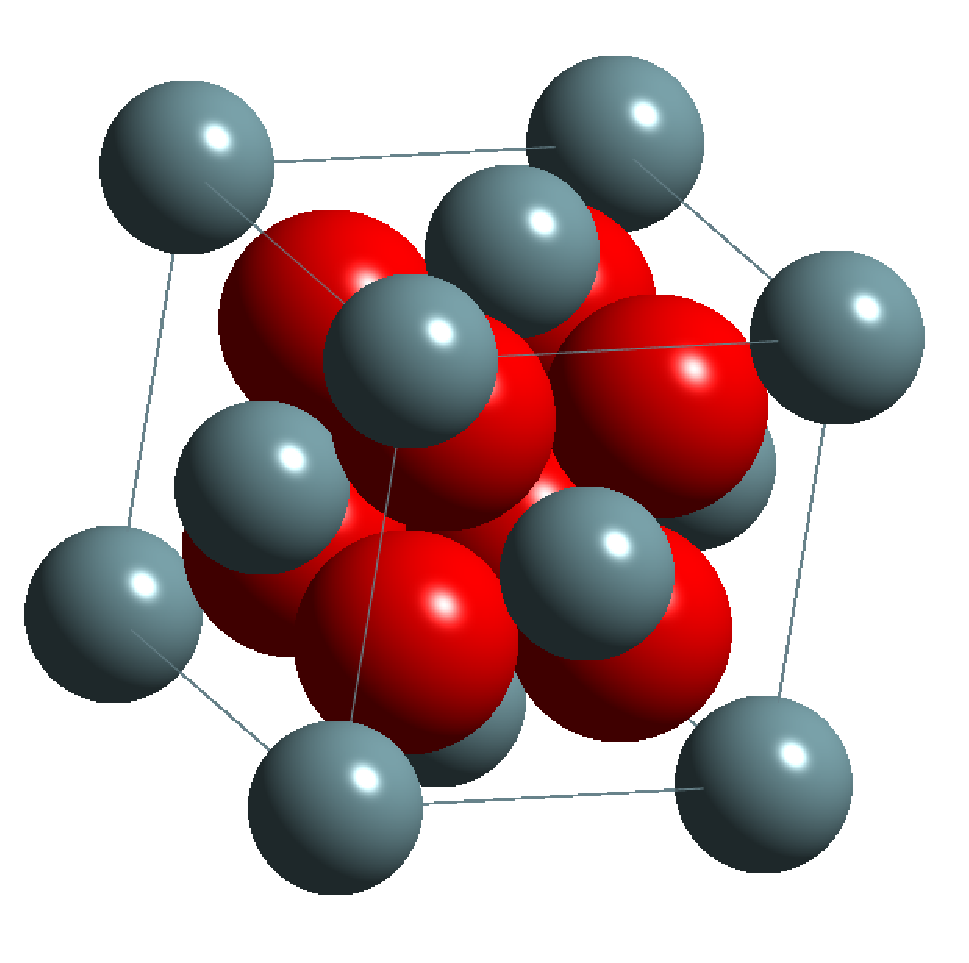
\includegraphics[scale=1.0]{Images/UO2}
\caption{\label{fig:uo2Lattice}An image representing the fluorite crystal structure.  For UO\textsubscript{2}, the smaller spheres indicate the uranium atoms, and the larger spheres indicate the oxygen atoms.  Image courtesy of the University of Cambridge under the Creative Commons license.}
\end{figure}

\section{Background\label{intro:background}}
Ceramics, metals, and polymers are composed of tiny crystals called \emph{grains}.  The orientation of each grain is generally independent of the orientation in the grains surrounding it, meaning there is a possibility (depending on how the crystal was formed\cite{callister2003}) that crystal structures will not line up at the interfaces where these two grains meet.  This ``atomic mismatch"\cite{callister2003} leads to broken or stretched atomic bonds where atoms will not be in the right place relative to a perfect crystal structure.  These defects are called grain boundaries (GBs), and an illustration of a GB can be seen in \Cref{fig:gb}. The most popular way to parameterize a GB is to use the five degree-of-freedom (DoF) model.\cite{patala2013, lejcek2010, homer2015, bulatov2014, harbison2015, rohrer2011}.  This model only uses the macroscopic DoFs (the observable degrees of freedom corresponding to the misorientation and inclination), ignoring the three translational DoFs (the ability of the grain to be translated or slid anywhere in space) possessed by each grain.  Three of the five DoFs specify the misorientation (or misaligment) of the grains with respect to each other.  The other two DoFs specify the orientation of the grain boundary plane (called the inclination).  The misorientation DoFs are the rotation angle $\theta$ (one of three) and the rotation axis (another two angles, where the first angle is measured in the $xy$-plane perpendicular to the $z$ axis, and the second angle is measured from the positive $z$-axis), while the inclination DoFs are defined by the normal of the grain boundary (two angles).\cite{lejcek2010}

There are three specific types of GBs that polycrystalline materials have: twist, tilt, and mixed GBs.\cite{lejcek2010, rohrer2011}  These GBs desribe the misorientation of two grains with respect to each other.  A twist boundary is when the axis of rotation between the two grains is parallel to the GB normal.  Tilt boundaries are composed of symmetric and asymmetric tilt boundaries.  A tilt boundary describes a boundary whose axis of rotation between the two grains is perpendicular to the GB normal.  Symmetric tilt boundaries describe a GB whose boundary plane is a mirror plane: one side of the boundary is the mirror of the other.  Thus, the angles between the boundary plane and the orientation axes of the two grains are equal. Asymmetric tilt is when the angles are not equal.  \Cref{fig:misorientation} shows a representation of tilt boundaries (top) and twist boundaries (bottom).  A mixed GB is a combination of twist and tilt boundaries in some degree.

Understanding GBs is important because of the effects they have on material properties.\cite{patala2013, homer2015, bulatov2014}  Extra energy is in the crystal structure because of the atomic mismatch at the boundaries.  This extra energy, called GB energy, gives rise to GB motion.  Knowing and predicting how the GBs will move allows for more accurate calculations of a material's properties.  Thus, GB energy needs to be fully understood in order to accurately model the evolution of material properties.

Two methods of modeling GB energy are the isotropic and anisotropic models.  The most common method (and easier method) is the isotropic model.  This model ignores the impact of inclination on the GB energy, and assumes that all inclinations for a given misorientation are equal, reducing the five-dimensional (5D) parameter space to a three-dimensional (3D) parameter space.  The reasons for assuming this model historically have been that it was assumed that the inclination had little or no impact on the GB energy, or (later) that it was too difficult to create a full five DoF model.\cite{homer2015}  Alternatively, there is the anisotropic approach.  This approach seeks to quantify the effect that misorientation \emph{and} inclination have on the GB energy.  Currently researchers acknowledge the need for a full five DoF model for the GB energy, but assert the difficulty inherent in developing such a model.\cite{rohrer2011, lejcek2010, homer2015}  Despite these difficulties, GB energy functions for certain materials, namely fcc metals copper, gold, aluminum, and nickel, have proven successful.\cite{bulatov2014}

\begin{figure}[ht!]
 \centering
 
 \subfloat[]{\label{fig:gb}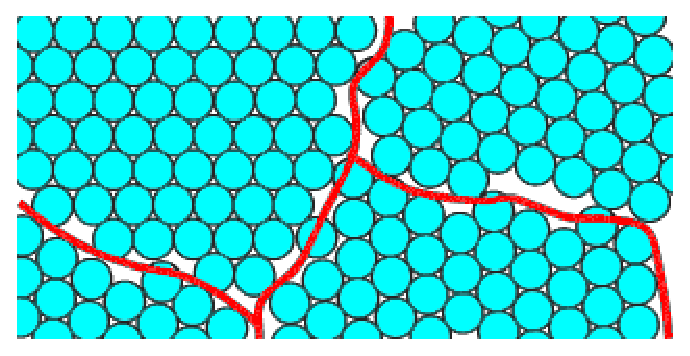
\includegraphics[scale=.9]{Images/grainBoundary}}\quad
 \subfloat[]{\label{fig:misorientation}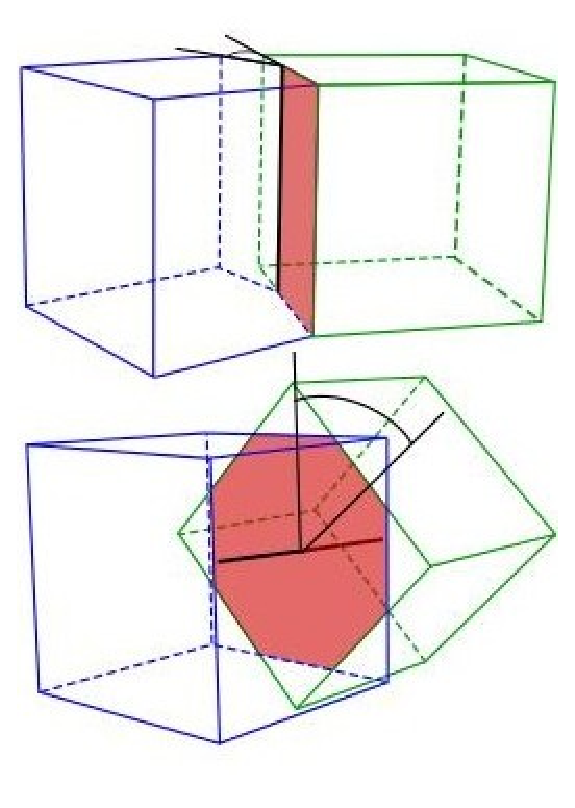
\includegraphics[scale=.6]{Images/twistTilt}}\quad
 \caption{\label{gbs} A representation of GBs, where \protect\subref{fig:gb} shows an example of a grain boundary and \protect\subref{fig:misorientation} shows an example of GB types.  In \protect\subref{fig:gb} individual atoms of the grains are the circles, while the grain boundary is highlighted by the line.  Atomic mismatch between the differently oriented grains causes an excess of energy to be present within the material, which has an effect on the material's properties.  Image courtesy of the University of Cambridge under the Creative Commons license. In \protect\subref{fig:misorientation} the axis of rotation for the tilt GB (top) is perpendicular to the GB normal, and for the twist GB (bottom) is parallel to the GB normal.  Image courtesy of Wikipedia under the Creative Commons license.}
\end{figure}

\section{Previous Work\label{intro:prevWork}}
Bulatov \emph{et al.}\cite{bulatov2014} developed a five DoF function which accurately interpolates GB energies for (certain?) fcc metals.  They used energies for GBs along specific axes to interpolate the full 5D space.  A more detailed explanation of their methods is presented in \Cref{methods}.  Harbison\cite{harbison2015} applied Bulatov \emph{et al.}'s methods to calculate similar parameters to describe the full five DoF GB space for UO\textsubscript{2}.  GB energies were gathered for various misorientations around a high-symmetry axis using molecular dynamics (MD) simulations.  The fitting procedure created a set of 43 parameters defining the function needed to interpolate an arbitrary GB energy.

%%%%%%%%%%%%%%%%%%%%%%%%%%%%%%%%%%%%%%%%%%%%%%%%%%%%%%%%%%%%%%%%%%%%%%%%%%%
% Does this need to go at the end of the "intro" section (before background?)
%%%%%%%%%%%%%%%%%%%%%%%%%%%%%%%%%%%%%%%%%%%%%%%%%%%%%%%%%%%%%%%%%%%%%%%%%%%
This work improves the fitting parameters by using MD results calculated by Zhang\cite{zhang2016} and Hansen\cite{hansen2016} with an anneal of 800K.  Harbison's data was not calculated with an anneal\cite{harbison2015}, which prevented the atoms from finding their ideal energetic minimum.  The 800 K anneal allows the atoms to relax to a value closer to their global minimum, as will be shown in \Cref{results}.  The energies from these simulations will be incorporated into a database that will be read into a  MATLAB\textsuperscript{\textregistered} script to fit the function parameters.  The updated parameters will be incorporated in Idaho National Laboratory's (INL's) mesoscale phase field modeling platform MARMOT for use in modeling nuclear fuels.  As these parameters are implemented in the modeling software, various tests of the UO\textsubscript{2} fuel can be performed to determine how the material properties change while in-reactor. 

\chapter{Methods\label{methods}}
Sufficient data is a requirement for any fitting procedure, but unfortunately there is a lack of data on UO\textsubscript{2} GB energies in the literature.  Molecular dynamics (MD) simulations\cite{zhang2016,hansen2016} were used as fitting data to calculate the GB energies of various lattices based on the coincident site lattice (CSL) model. This model is built off of the idea that GB energy is low when more lattice sites are in coincidence.  A number defined as the $\Sigma$-number (pronounced ``sigma-number" (????))describes the number of coincident sites per total number of lattice sites in a given unit cell of a crystal.\cite{lejcek2010, rohrer2011} A MATLAB\textsuperscript{\textregistered} script, developed using Bulatov \emph{et al.}'s methods\cite{bulatov2014} and building off of Harbison's\cite{harbison2015} script used the gathered data.

%The data gathered was put into a MATLAB\textsuperscript{\textregistered} script developed using Bulatov \emph{et al.}'s methods\cite{bulatov2014} and building off of Harbison's\cite{harbison2015} script.  A reduced chi-square statistic was calculated to determine the effectiveness of the fit.

\section{Molecular Dynamics\label{methods:MD}}
Simulation results from the Large-scale Atomic/Molecular Massively Parallel Simulation (LAMMPS) software (developed at Sandia National Laboratory\cite{plimpton1995}) were gathered for a number of twist, tilt, and mixed GBs.  These calculations were performed by creating two crystals of UO\textsubscript{2} and placing them together in various orientations.  A GB is introduced at the interface, creating GB energy.  The energy of the system is calculated from the interatomic forces inside the crystal.  That energy is compared to the energy of a single grain (of the same size as the combined two grains) of UO\textsubscript{2} in order to determine the energy at the GB.\cite{harbison2015}  The difference between these two values divided by twice the area of the GB gives the GB energy of the particular misorientation.\cite{butterfield2013} An example of how the atoms align is shown in \Cref{fig:lammps}. Harbison's original calculations\cite{harbison2015} were done using no anneal (maximum temperature was approximately 0K), only allowing the atoms to relax to their local minima.  This work used an anneal of 800K, % NOTE: Why was 800K chosen?
allowing the atoms to relax to a better estimate of their global minimum value as is shown in \Cref{fig:100,fig:110,fig:111}.  
The misorientation angles at which these energies were calculated were the same as used in the work of Harbison.  These energies are used in the fitting procedure to produce parameters describing the five-dimensional GB space.
% This section needs more info, I just don't know what yet.  Mostly on MD information.  That would require some discussion with Yongfeng and Evan.

\begin{figure}[ht!]
 \centering
 
 \subfloat[]{\label{fig:lammps1}\includegraphics[scale=0.287]{"Images/LAMMPS example image"}}\quad
 \subfloat[]{\label{fig:lammps2}\includegraphics[scale=0.3]{"Images/LAMMPS example image2"}}\quad
 \caption{\label{fig:lammps}These figures demonstrate example crystal structures of UO\textsubscript{2} after an annealing process.  The better the atoms line up, the lower the energy is. \protect\subref{fig:lammps1} shows an example of a mostly aligned GB, indicative of a lower energy.  \protect\subref{fig:lammps2} shows an example of a misaligned GB, indicative of a higher energy.  These two images are from a \textlangle{}111\textrangle{} twist image.  Different viewpoints show different amounts of alignment.  The LAMMPS simulation package takes care of all the calculations to determine the energy at these GBs. Images courtesy of Dr. Evan Hansen, used with permission.}
\end{figure}

\section{Bulatov \emph{et al.}'s Methods\label{methods:bulatov}}
In order to find the energy of an arbitrary GB in the five-space, Bulatov \emph{et al.}\cite{bulatov2014} implemented a hierarchical interpolation method.  They started by choosing three three-dimensional (3D) high-symmetry axes to use as scaffolding to build the entire five-dimensional (5D) function.  The axes chosen were the \textlangle{}100\textrangle{}, \textlangle{}110\textrangle{}, and the \textlangle{}111\textrangle{} sets for their four-, two-, and three-fold rotational symmetries respectively.\footnote{For cubic crystals, rotations of 90\textdegree{}, 180\textdegree{}, or 120\textdegree{} about any \textlangle{}100\textrangle{}, \textlangle{}110\textrangle{}, or \textlangle{}111\textrangle{} axis respectively is a symmetry operation.\cite{stokes2007}  Thus, the \textlangle{}100\textrangle{} set is four-fold symmetric (360\textdegree{}$/90$\textdegree{}$=4$), the \textlangle{}110\textrangle{} set is two-fold symmetric (360\textdegree{}$/180$\textdegree{}$=2$), and the \textlangle{}111\textrangle{} set is three-fold symmetric (360\textdegree{}$/120$\textdegree{}$=3$).}  Each 3D subset is built from an interpolation of their own one- and two-dimensional subsets.  The symmetric tilt and twist GBs for each set were fitted first because of their simplicity.  Only the rotation angle is needed to fully define the energies for these subsets, making them one-dimensional (in \Cref{fig:bulatov5D}, the darker bands in the smaller circles).  From the symmetric tilt subset, the asymmetric, or general, tilt subset was interpolated.  A second rotation angle defining the rotation of the second grain makes this subset two-dimensional (the lighter, wider band of color around the symmetric subset).  A combination of the general tilt subset (two dimensions) and the twist subset (one dimension) was used to interpolate the 3D subset for each high-symmetry axis (the three smaller circles).  These three 3D subsets were then used to interpolate the GB 5D space.

Read and Shockley\cite{read1950} initially developed the equations used to do the interpolation (called Read-Shockley functions) to describe the GB energy at low-angle boundaries (The definition of a ``low-angle boundary" varies from material to material.  Boundaries with angles higher than\cite{rohrer2011} 6\textdegree{} up to\cite{wolf1989} 15\textdegree{} have been cited as low-angle boundaries).  Wolf developed a method\cite{wolf1989} using Read-Shockley functions to calculate the energies at high-angle boundaries, with the resulting functions being called Read-Shockley-Wolf (RSW) functions.  These RSW functions take the form:
\begin{equation}
E_{min} + (E_{max} - E_{min})\ \textnormal{sin}\left(\frac{\pi}{2}\frac{\theta-\theta_{min}}{\theta_{max} - \theta_{min}}\right)\left(1-a\textnormal{log}\left(\textnormal{sin}\left(\frac{\pi}{2}\frac{\theta-\theta_{min}}{\theta_{max} - \theta_{min}}\right)\right)\right),
\end{equation}
where $\theta$ is the misorientation angle, $\theta_{min}$ is the minimum angle on the domain, $\theta_{max}$ is the maximum angle on the domain, and $a$ is a shaping parameter.  Each of Wolf's RSW functions cover a ``low-angle" subset of the domain of the 1D GB space.  An example of a simple RSW function is shown in \Cref{fig:RSW}.  Multiple RSW functions are stitched together to form the 1D subsets.

\begin{figure}[ht!]
 \centering
 \subfloat[]{\label{fig:bulatov5D}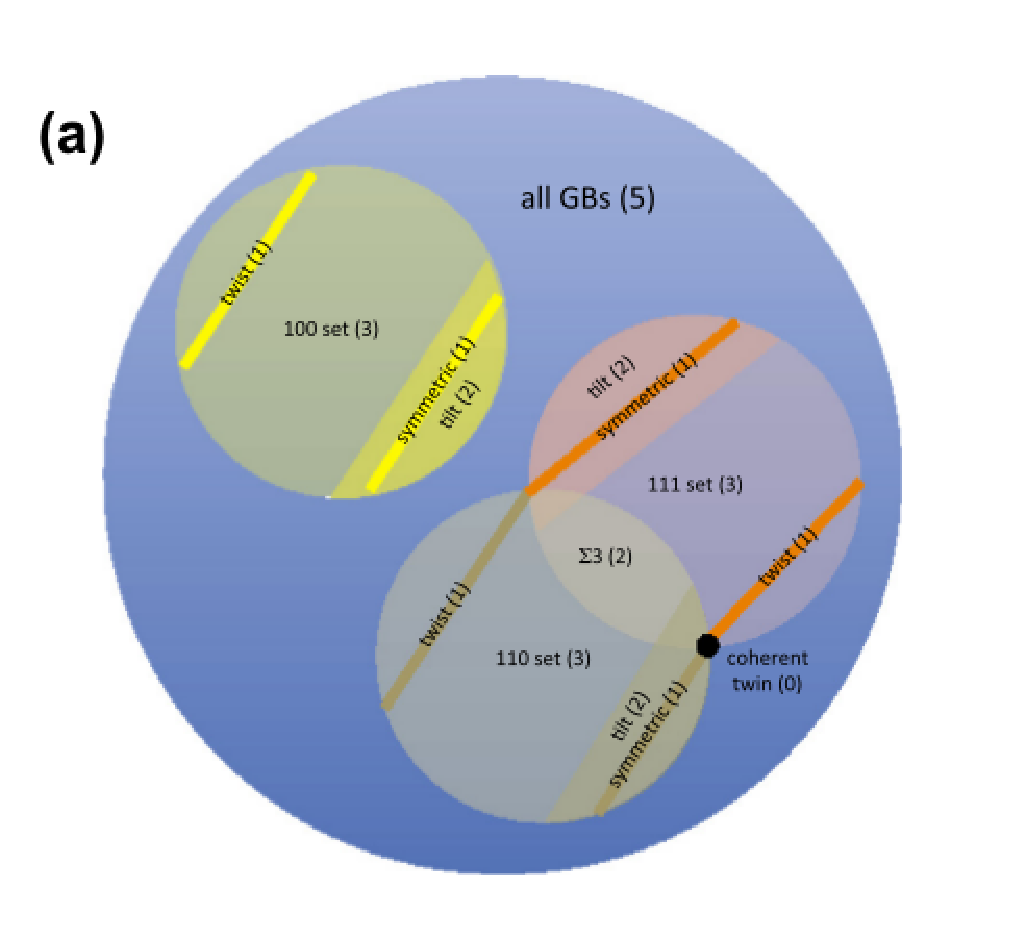
\includegraphics[scale=0.42]{Images/bulatov_5D_model}}\quad
 \subfloat[]{\label{fig:bulatovRodrigues}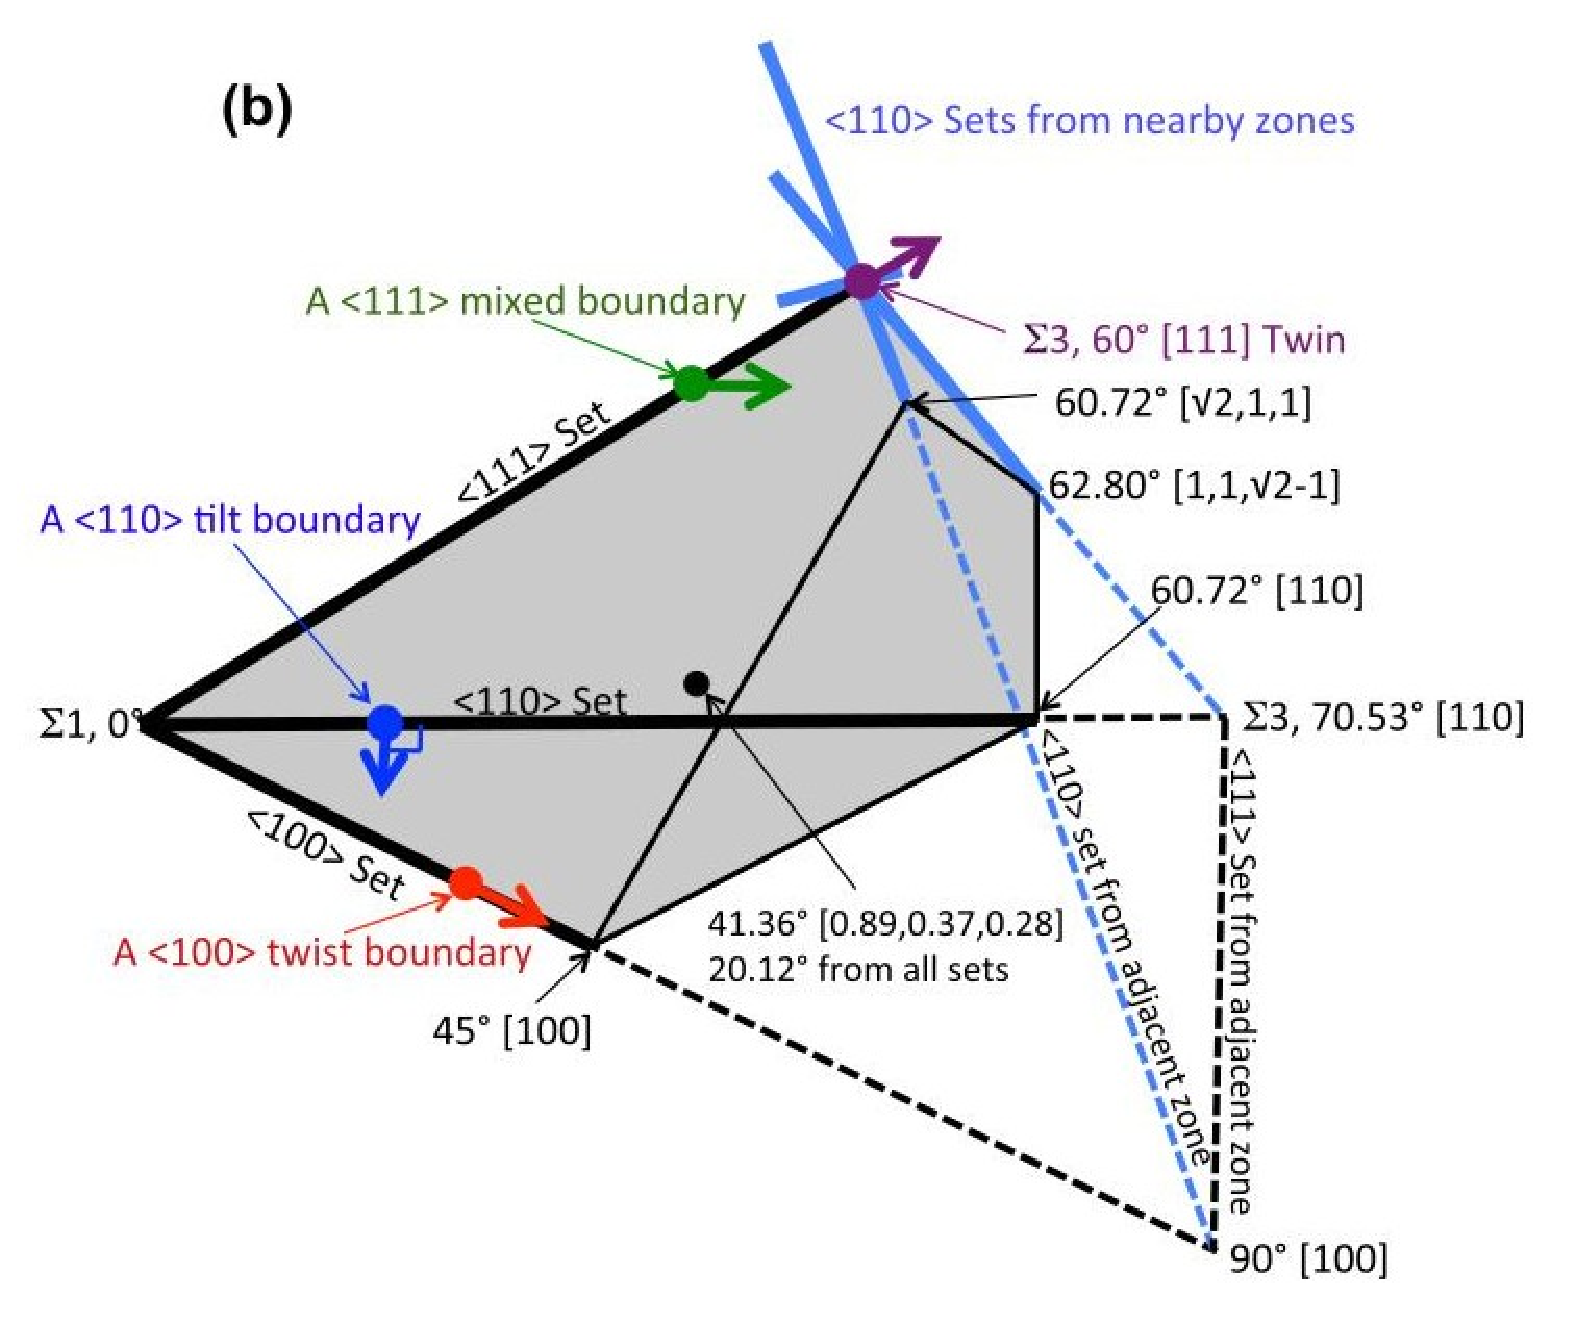
\includegraphics[scale=0.32]{Images/bulatov_rodrigues}}
 \caption{\label{fig:bulatovFig2}Figure 2 from Bulatov \emph{et al.}\cite{bulatov2014}. \protect\subref{fig:bulatov5D} demonstrates the theoretical relationship between the high-symmetry subsets of the 5D GB space.  Each multi-dimensional subset is interpolated from smaller-dimensional subsets. \protect\subref{fig:bulatovRodrigues} shows the Rodrigues space representation of the fundamental zone of all GBs as built from three high-symmetry axes (\textlangle{}100\textrangle{}, \textlangle{}110\textrangle{}, and \textlangle{}111\textrangle{}).  The unit vectors along the axis identify the boundary plane inclination in the frame of grain one.  A parallel vector thus represents a twist boundary, a perpendicular vector represents a tilt boundary, and neither parallel nor perpendicular vectors represent a mixed boundary.  The full misorientation space has 1152 symmetrically equivalent copies of the fundamental zone\cite{bulatov2014, randle2000} which allows the infinite nature of Rodrigues space to be accounted for.}
\end{figure}

\begin{figure}[ht!]
 \centering
 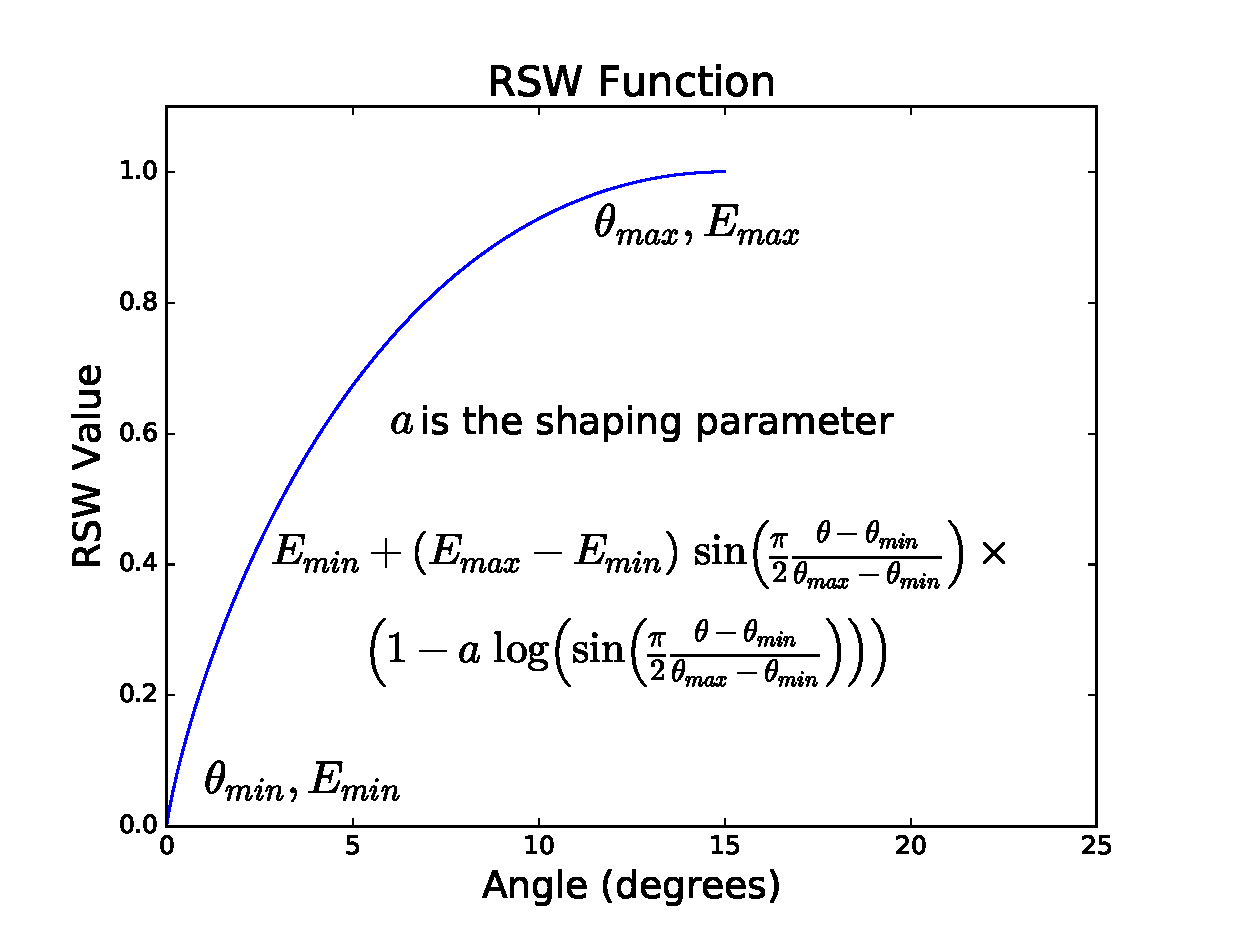
\includegraphics[scale=0.5]{Images/rsw}
 \caption{\label{fig:RSW}An example of an RSW function with $\theta_{min} = 0$\textdegree{}, $\theta_{max} = 15$\textdegree{}, and $a$ (the shaping parameter) $= 0.5$  Combining these functions into a Piecewise set over a given domain gives the GB energy curves their distinct, cusp-like behavior.  The RSW functions are scaled using $E_{min}$ and $E_{max}$.  In this example, $E_{min} = 0$ and $E_{max} = 1$.}
 % NOTE!!! using \degree WILL NOT WORK!
\end{figure}

\section{Representations of Grain Boundary Space\label{methods:GBReps}}
Part of the development of this 5D function was accomplished through visual representations of the GB space.  However, the size of the five-space in which GBs reside makes representing them difficult.  Different methods have been developed to represent them, each with their advantages and disadvantages.  Three of these methods are the axis-angle representation, the Rodrigues representation, and the fundamental zone representation.  These methods, though described separately, can be used together to form a better picture of what the GB space looks like (see for example \Cref{fig:bulatovRodrigues} which combines the Rodrigues representation and the fundamental zone representation).

\subsection{Axis-Angle Representation\label{GBReps:AA}}
The axis-angle representation is the simplest of the three described here.  The axis of rotation of the GB specifies the point in axis-angle space, and the angle of misorientation between the two grains at the GB specifies the magnitude of the vector.  Thus, the axis ($\bm{a}$, where $\bm{a}$ has components $a_x$, $a_y$, and $a_z$) and the angle ($\theta$) mathematically represent an axis-angle vector as:
\begin{equation}
\bm{A} = \bm{a}\ \theta
\label{eq:aaVec}
\end{equation} 

The axis-angle space can only take into account three degrees of freedom: the two angles specifying the axis, and the angle rotated through.  Thus, axis-angle space cannot fully visualize all of the necessary information contained in the full 5D space.\cite{frank1988} An added difficulty of using this representation is its infinite space because it is a mapping of an axis and an angle onto a Cartesian coordinate system.  This mapping means understanding the entire GB space is nearly impossible without the help of additional methods.  The axis-angle representation is best used as a starting point to move to other, more robust representations, and to represent the misorientation between two grains.\cite{randle2000}

\subsection{Rodrigues Representation\label{GBReps:Rodrigues}}
The Rodrigues representation (sometimes called the ``Rodrigues-Frank" representation) uses Rodrigues vectors to represent rotations in Rodrigues space.  This representation takes ideas from the axis-angle space, but makes a few changes allowing crystal symmetries to be taken into account.  The axis about which a GB is oriented still specifies the point in space, but the tangent of half the angle represents the magnitude of the vector. Thus, a Rodrigues vector can be represented as:\cite{morawiec1996, becker1989, frank1988, randle2000, priester2013}
\begin{equation}
\bm{R}=\bm{a}\ \textnormal{tan}\left(\frac{\theta}{2}\right)
\label{eq:rodriguesVec}
\end{equation}
Some researchers favor this representation over others because of the lack of curvature such a mapping entails.\cite{frank1988, randle2000}  However, still only three of the five degrees of freedom are specified.  A unit vector at the points along the axis represents the other two in \Cref{fig:bulatovRodrigues}. A parallel vector represents a twist boundary, and a perpendicular vector represents a tilt boundary.  Anything else represents a mix of twist and tilt (or a mixed boundary).  One difficulty in using Rodrigues space is it also is an infinite space, as it simply maps an axis and an angle onto a Cartesian coordinate system.\cite{frank1988, kirch2008}.

\subsection{Fundamental Zone Representation\label{GBReps:FunZone}}
The fundamental zone is perhaps the best graphical representation for the 5D GB.  This representation takes advantage of the symmetries inherent in crystals\cite{stokes2007} to simplify an infinite space into a compact, finite area called the fundamental zone.\cite{bulatov2014, patala2013, homer2015, morawiec1996, patala2012}  Every point within the space represents a unique orientation, and every point outside the space can be represented as a point inside the space through symmetry operations.\cite{morawiec1996, becker1989, frank1988}  Bulatov \emph{et al.} used this idea in connection with Rodrigues space to create \Cref{fig:bulatovRodrigues}.  In Rodrigues space, the crystal symmetric of the material determine the shape of the fundamental zone.\cite{patala2013, morawiec1996}  For fcc crystals, the fundamental zone takes the form of a truncated tetrahedron.\cite{bulatov2014}  The edges of the fundamental zone in Rodrigues space represent the high-symmetry rotation axes, and points on one face can represent another point on a different face of the fundamental zone.  

\section{Code Analysis\label{methods:code}}
Harbison's\cite{harbison2015} and Bulatov \emph{et al.}'s\cite{bulatov2014} MATLAB\textsuperscript{\textregistered} scripts were used in this work.  These codes were analyzed to understand the process for both fitting the GB energy parameters, and for calculating the GB energy of an arbitrary GB.
\subsection{The Fitting Code\label{code:fitting}}
An extensive analysis of Harbison's\cite{harbison2015} code was conducted to learn how it worked.  The basic outline for how the fit occurs is as follows.  First, data is read in from a database containing energies associated with either a twist or tilt GB on one of the three high-symmetry axes.  Test parameters which are used as starting points are also read in from a separate database.  The one-dimensional sets are fitted first because of their simplicity.  The parameters found from the 1D fits are used in fitting the higher-dimensional sets.  Important angles are specified where low energies are expected, such as the $\Sigma5$ boundary for the \textlangle{}100\textrangle{} symmetric tilt subset.  These angles are calculated based on the $\Sigma$-number from CSL theory. Because the $\Sigma$-number designates how many lattice points  are between each coincident site (and assuming that the space between each lattice site, the lattice constant, is known) the angle of the GB misorientation can be determined.  In order to minimize the potential for error in calculations, every energy in the parameter-vector is listed as a scaled value based on the $e_{RGB}$ parameter -- a parameter representing the energy of an arbitrary, random GB, and can be seen as an average of the GB energies.  Thus, to make relevant comparisons, the energies are unscaled based on the units of energy desired (typically J/m\textsuperscript{2}).  An initial step size is then set, and data for the specific subsets is read in from a database.  All of the parameters and the angle-energy pairs are then passed into a grid-search fitting function.  Each subset had a different initial step size to avoid a numerical error where the steps would take the angles currently being looked at outside of their domain. % NEEDS CLARIFICATION

Once the six one-dimensional subsets and the three two-dimensional subsets are fitted, the three-dimensional subsets are fitted using the twist and asymmetric tilt subsets to calculate the mixing parameters (defining the relationship between the twist and general tilt subsets within a high-symmetry axis - i.e. the relationship between the small dark bands representing the twist boundaries and the lighter, wider bands representing the tilt boundaries in \Cref{fig:bulatov5D}).  The final step is to calculate the weighting parameters, which defines the relationship between the three high-symmetry subsets.  Equations defining the various relationships can be found in Bulatov \emph{et al.}'s work.

% I need to make sure I explain the difference between how the grid-search is calculating chi squared and how I calculated chi squared for our fit.  I should look into how Bulatov calculated his chi squared statistic.

\subsection{The Energy Calculation Code\label{code:energyCalc}}
Bulatov \emph{et al.}'s open-source MATLAB\textsuperscript{\textregistered} code\cite{bulatov2014} calculates the energy of an arbitrary GB in an fcc metal. The same procedure is used for calculating an arbitrary GB in uranium dioxide, and goes as follows.  First, metrics defining the ``distance" between the GB and all three high-symmetry axes are calculated.  These distances are calculated by looking at all symmetrically equivalent representations of a GB on a per-axis basis (for cubic crystals, there are 24 equivalent representations\cite{stokes2007}).  Because there are three, six, and four unique axes for the \textlangle{}100\textrangle{}, \textlangle{}110\textrangle{}, and \textlangle{}111\textrangle{} axes respectively, a maximum of $6\times24=144$ distances are calculated.  Those distances exceeding a predefined cutoff distance are discarded.  After all distances have been calculated, only the unique representations are kept to avoid double-counting certain representations.\cite{bulatov2014}  Energies are calculated for each unique distance in each subset.  These energies are then weighted and summed together to give the interpolated energy for the specified GB. % This paragraph needs additional explanation on what the distances are.  I also use the phrase "Th[oe]se distances..." way too much.  This needs to be changed.

\section{Reduced Chi-Square Statistic\label{methods:chi2}}
A good way to test how well a function fits the data is to use a reduced chi-square goodness-of-fit statistic.\cite{bevington2003}  In order to calculate this statistic the orientation matrices (which Bulatov \emph{et al.} calls the P and Q matrices for the first and second grain respectively) were needed as input parameters to Bulatov \emph{et al.}'s function.  These three by three matrices specify the orientation in a lab frame of the two grains individually. A good fit will have a reduced chi-square value close to one, while those values greater than one indicate an under fit, and those values less than one indicate an over fit.\cite{bevington2003}
\subsection{Developing the P and Q Matrices\label{chi2:PQ}}
% This is going to need some major revisions
Creating the P and Q matrices was a non-trivial task.  Because there has been so much work done with crystallography over the past few decades, many different methods have been developed to specify the orientation matrices of grains. A rotation matrix also needed to be calculated which rotates the axis of rotation to the [100] direction, as Bulatov \emph{et al.}'s energy calculation code assumes.  Three methods, following the method prescribed in MARMOT, using the Rodrigues rotation formula, and using the Bunge rotation matrix were used in the process of developing these matrices are described below.

\subsubsection{MARMOT Method\label{PQ:MARMOT}}
MARMOT, Idaho National Laboratory's (INL's) mesoscale phase-field modeling platform,\cite{tonks2012} calculates the P and Q matrices for the grains using Euler angles as input parameters.  The Euler angles are converted to the orientation matrices using the Bunge convention, i.e. the $ZXZ$ or $ZX'Z''$ rotation, where the first rotation is about the \emph{z} axis, the second rotation is around the new \emph{x} axis, and the final rotation is about the new \emph{z} axis.  The formula for this conversion from Bunge Euler angles to the rotation matrix is found by multiplying the \emph{z}, \emph{x}, and \emph{z} rotation matrices together in that order to get:

\begin{equation}
\label{eq:bungeMat}
\left[
\begin{array}{ccc}
c_1\ c_3 - c_2\ s_1\ s_3 & -c_1\ s_3 - c_2\ c_3\ s_1 & \phantom{-}s_1\ s_2 \\
c_3\ s_1 + c_1\ c_2\ s_3 & \phantom{-}c_1\ c_2\ c_3 - s_1\ s_3 & -c_1\ s_2 \\
s_2\ s_3 & \phantom{-}c_3\ s_2 & \phantom{-}c_2 
\end{array}
\right]
\end{equation}
where $c_\textnormal{n}$ and $s_\textnormal{n}$ represent the cosine and sine of the respective angles (1 represents the first \emph{z} rotation, 2 represents the \emph{x} rotation, and 3 represents the second \emph{z} rotation.  These angles are usually referred to as\cite{randle2000} $\varphi_1$, $\Phi$, $\varphi_2$).

The rotation matrix was calculated in MARMOT by using the GB normal and finding the rotation matrix required to rotate that vector to the [100] direction.  In MARMOT, simulations are set up through input files.  In the input files there are different sections (called blocks) specifying material parameters, boundary conditions, initial conditions, and what physics to use to solve the problem (among others).  The initial condition used to calculate the rotation matrices in MARMOT was a horizontal or vertical line for tilt or twist boundaries respectively.  Because of this set up, the GB normals were either along the [010] axis for the tilt boundaries, or [$\bar{1}$00] for twist boundaries.

\subsubsection{Rodrigues Rotation Formula\label{PQ:RRF}}
The Rodrigues rotation formula\cite{belongie2006} (RRF) is a way of calculating the rotation matrices given an axis and an angle using the following formula:
\begin{equation}
\label{eq:rrf}
\bm{R} = \bm{I} + \textnormal{sin}\ \theta\ \bm{K} + (1 - \textnormal{cos}\ \theta)\ \bm{K}^2,
\end{equation}
where $\bm{I}$ is the 3x3 identity matrix, $\theta$ is the angle rotated through, and $\bm{K}$ is the skew-symmetric matrix formed by the axis of rotation ($\bm{a}$) by:
\begin{equation}
\label{eq:skewSymMat}
\left[
\begin{array}{ccc}
\phantom{-}0 & -a_z & \phantom{-}a_y \\
\phantom{-}a_z & \phantom{-}0 & -a_x \\
-a_y & \phantom{-}a_x & \phantom{-}0
\end{array}
\right]
\end{equation}

The rotation matrices were calculated two different ways with this orientation matrix formulation.  One method was to simply use the MARMOT-generated rotation matrices.  These rotation matrices Another method was to calculate the rotation matrices using geometric arguments (see \Cref{fig:PlaneNorms}).  From these arguments the normals are identified in \Cref{table:geometricgbnorms}.

\begin{figure}[ht!]
\begin{minipage}{0.33\linewidth}
 \centering
 \subfloat[]{\label{fig:100TwistPlane}\includegraphics[scale=0.2]{Images/Twist100Plane}}
\end{minipage}%
\begin{minipage}{0.33\linewidth}
 \centering
 \subfloat[]{\label{fig:110TwistPlane}\includegraphics[scale=0.2]{Images/Twist110Plane}}
\end{minipage}%
\begin{minipage}{0.33\linewidth}
 \centering
 \subfloat[]{\label{fig:111TwistPlane}\includegraphics[scale=0.2]{Images/Twist111Plane}}
\end{minipage}
 \centering
 
 \subfloat[]{\label{fig:100TiltPlane}\includegraphics[scale=0.2]{Images/Tilt100Plane}}\quad
 \subfloat[]{\label{fig:110TiltPlane}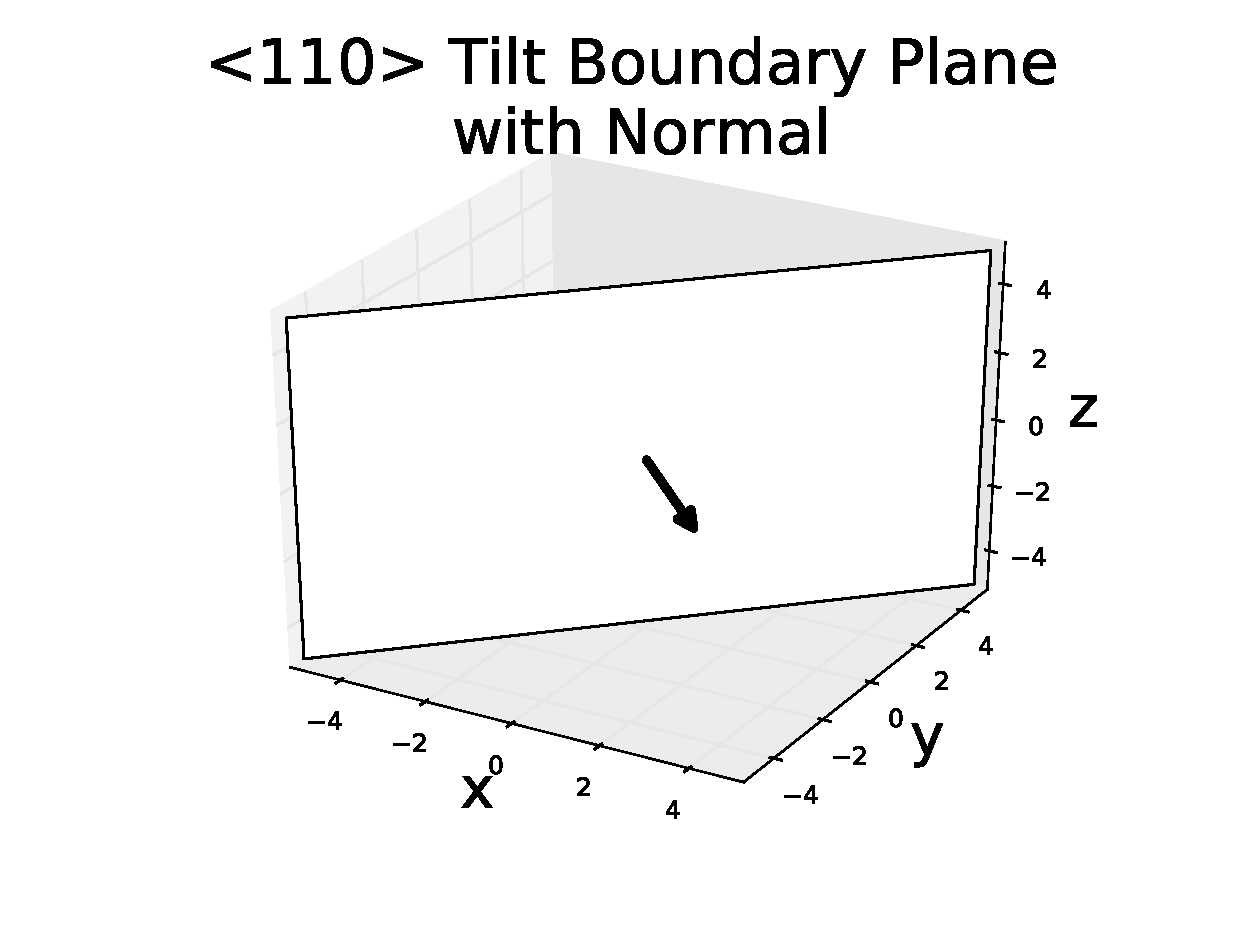
\includegraphics[scale=0.2]{Images/Tilt110Plane}}\quad
 \caption{\label{fig:PlaneNorms}A geometric method of determining the normals of a GB.  \protect\subref{fig:100TwistPlane} to \protect\subref{fig:111TwistPlane} show the GB normals for a GB perpendicular to the axis of rotation (a twist GB).  The GB normal is simply the axis about which the grains are rotated. \protect\subref{fig:100TiltPlane} and \protect\subref{fig:110TiltPlane} show the GB normals for a GB parallel to the axis of rotation (a tilt GB).  The GB normal is perpendicular to the axis of rotation.  The same GB normal for \textlangle{}110\textrangle{} Tilt can be used for \textlangle{}111\textrangle{} Tilt.}

\end{figure}

\begin{table}[ht!]
\centering
\caption{\label{table:geometricgbnorms}Table of GB normals for different GB types. The normalized dot product of the axis with the GB normal is zero in all tilt cases and one in all twist cases.  There are two options for the grain boundary normals of each subset because of inversion symmetries.}

\begin{tabular}{ccc}
Axis & Boundary Type & GB Normal \\
\hline
\hline
\multirow{2}{*}{\textlangle{}100\textrangle{}} & \multirow{2}{*}{Tilt} & [010] \\
                              & & [0$\bar{1}$0] \\
\hline
\multirow{2}{*}{\textlangle{}110\textrangle{}} & \multirow{2}{*}{Tilt} & [1$\bar{1}$0] \\
							  & & [$\bar{1}$10] \\
\hline
\multirow{2}{*}{\textlangle{}111\textrangle{}} & \multirow{2}{*}{Tilt} & [1$\bar{1}$0] \\
							  & & [$\bar{1}$10] \\
\hline
\multirow{2}{*}{\textlangle{}100\textrangle{}} & \multirow{2}{*}{Twist} & [100] \\
							  & & [$\bar{1}$00] \\
\hline
\multirow{2}{*}{\textlangle{}110\textrangle{}} & \multirow{2}{*}{Twist} & [110] \\
							  & & [$\bar{1}\bar{1}$0] \\
\hline
\multirow{2}{*}{\textlangle{}111\textrangle{}} & \multirow{2}{*}{Twist} & [111] \\
							  & & [$\bar{1}\bar{1}\bar{1}$] \\
\hline
\hline
\end{tabular}
\end{table}

\subsubsection{Bunge Rotation Matrix\label{PQ:BungeMat}}
The Bunge rotation matrix (see \Cref{eq:bungeMat}) is what MARMOT uses to create the orientation matrices.  There were various methods used to calculate the Euler angles, of which three are briefly described here. The Euler angles (once calculated) were used in the first two methods to calculate the entirety of the rotation matrix.

The first method tried was to use scripts developed to calculate the various Euler angles for MARMOT.  These scripts did not work because of the same assumptions made earlier about the orientation of the GB, namely, that all pure tilt GBs have a normal of 010, and that all pure twist GBs have a normal of $\bar{1}$00.  The difference between MARMOT's boundary conditions and the boundary conditions of this work is that GBs in this work are assumed to be either perpendicular or parallel to the rotation axis, as opposed to always being along the x or y axis.

The second method was to use an open-source MATLAB\textsuperscript{\textregistered} package called MTEX.\cite{bachmann2010}  This package calculates Euler angles using quaternions.  These Euler angles did not generate the correct results either, for the most part creating the same sorts of graphs as the MARMOT method.  It is uncertain why this method did not work.

The working method used the mathematics of quaternions.\cite{weisstein2004}  The quaternions were calculated directly based on the misorientation axis and angle.  A quaternion is a four-dimensional vector containing one real part, and three imaginary parts.  The components of the vector are calculated as follows:
\begin{equation}
\label{eq:quat}
\bm{q}=\left[\textnormal{cos}\left(\frac{\theta}{2}\right),\ a_x\,\textnormal{sin}\left(\frac{\theta}{2}\right),\ a_y\,\textnormal{sin}\left(\frac{\theta}{2}\right),\ a_z\,\textnormal{sin}\left(\frac{\theta}{2}\right)\right],
\end{equation}
with axis $\bm{a}$ and misorientation angle $\theta$.  Once the axis and misorientation angle are converted to a quaternion, another conversion from a quaternion to the Bunge Euler angles is performed.  The angles are calculated using the \verb!atan2! method which allows for all four quadrants in the Cartesian space to be accounted for.  The angles are calculated using the following formulas:
\begin{align}
\label{eq:quat2euler}
\begin{aligned}
\chi &= \sqrt{(q_0^2+q_3^2)(q_1^2+q_2^2)}\\
\varphi_1 &= \textnormal{atan2}\left(\frac{q_0q_2+q_1q_3}{2\chi}, \frac{q_0q_1-q_2q_3}{2\chi}\right)\\
\Phi &= \textnormal{atan2}\left(2\chi, q_0^2+q_3^2-q_1^2-q_2^2\right)\\
\varphi_2 &= \textnormal{atan2}\left(\frac{q_1q_3-q_0q_2}{2\chi}, \frac{q_0q_1+q_2q_3}{2\chi}\right).
\end{aligned}
\end{align}
Once the Euler angles were calculated, they were put into \Cref{eq:bungeMat}, and the resulting matrices were used as the orientation for the grains.  The codes used to generate the orientation matrices can be found in \Cref{app:OrientationMatrix,app:genOrientationMatrix}.

\subsubsection{Testing The Matrices\label{PQ:Testing}}
In order to test the different methods, an attempt was made to reproduce the 1D subset graphs as shown in Bulatov \emph{et al.}.  Various levels of success were observed for the different methods.  The matrices giving the best results are shown in \Cref{fig:compare100,fig:compare110,fig:compare111}.


While the first method works well for MARMOT, the challenge accompanying its use was that MARMOT specifies a specific GB normal with the set up of the problem that is not necessarily what the MATLAB\textsuperscript{\textregistered} script expects.  Thus, the results coming from using this combination of matrices ended up working only for the \textlangle{}100\textrangle{} tilt, \textlangle{}110\textrangle{} tilt, and \textlangle{}100\textrangle{} twist subsets, while the \textlangle{}110\textrangle{} twist had issues with singularities, and the \textlangle{}111\textrangle{} subsets did not remotely match the expected outcome.

\subsection{Calculating Reduced Chi Squared\label{chi2:chi2red}}
There were two methods used to calculate the $\chi^2_{red}$ statistic.  The first method was to use the P and Q matrices as developed above to test the entirety of the fit.  The second method was to calculate the statistic for each 1D subset, then calculate the full $\chi^2_{red}$ value using the statistics from the subsets.  Results from these calculations are discussed in the next chapter.

The test for the entire fit was done using the P and Q matrices to calculate the energy in 1\textdegree{} intervals for each subset, using the \verb!GB5DOF.m! script.  The difference between the calculated values and the MD values was calculated, and the $\chi_{\textnormal{red}}^2$ value was calculated for each subset and for the entire fit, producing the results in \Cref{table:chi2} under the 800 K anneal column under the ``$\chi_{\textnormal{red}}^2$ using P and Q matrices" section.

Using the second method, the same angles used in the fitting procedure were used in the RSW equations creating the 1D subsets.  The differences between the values resulting from there and the MD simulation values lead to the $\chi_{\textnormal{red}}^2$ values shown in the 800 K anneal column under the $\chi_{\textnormal{red}}^2$ comparing the 1D fits section.  The same methods were implemented to calculate the $\chi_{\textnormal{red}}^2$ values for the data without an anneal.

The statistic calculated using these methods is different from the $\chi^2$ statistic used in the grid-search function.  The grid search used \Cref{eq:chi2grid}, and generated values of the same order as \Cref{eq:chi2}.

\begin{equation}
\label{eq:chi2grid}
\chi^2=\sum (E_{\textnormal{measured}} - E_{\textnormal{calculated}})^2
\end{equation}

\chapter{Results and Discussion\label{results}}
\section{Validation of P and Q Matrices\label{results:PQValid}}
The energy profiles calculated from the P and Q matrices were compared with the copper energy profiles expected from the parameters defined in Bulatov \emph{et al.}'s code to validate the generated P and Q matrices.  Results from this comparison for the \textlangle{}100\textrangle{} set are shown in \Cref{fig:compare100}, with all six subsets shown in \Cref{appfig:compare100,appfig:compare110,appfig:compare111}.  The calculated energies match exactly the predicted values for all but a few points.  Each data set mismatches the expected energy at 1\textdegree{}, and the tilt data sets also see this mismatch at their second to last data point.

\begin{figure}[ht!]
 \centering
 
 \subfloat[]{\label{fig:compare100Twist}\includegraphics[scale=0.24]{Images/TestPQFit100Twist}}\quad
 \subfloat[]{\label{fig:compare100Tilt}\includegraphics[scale=0.26]{Images/TestPQFit100Tilt}}
 \caption{\label{fig:compare100} The \textlangle{}100\textrangle{} twist \protect\subref{fig:compare100Twist} and tilt \protect\subref{fig:compare100Tilt} results for the P and Q matrices as compared to Bulatov \emph{et al.}'s energy profiles. The expected value was calculated using Bulatov \emph{et al.}'s \lstinline!GB5DOF.m! MATLAB\textsuperscript{\textregistered} script with the default values.  The calculated values were found by inputting the matrices into the \lstinline!GB5DOF.m! script. With the exception of the data points at 1\textdegree{} in both \protect\subref{fig:compare100Twist} and \protect\subref{fig:compare100Tilt} and 89\textdegree{} in \protect\subref{fig:compare100Tilt}, the energies calculated from the matrices matches the expected curves exactly.}
\end{figure}

\section{Fitting Results\label{results:fit}}
Comparisons for the 1D results from Harbison\cite{harbison2015} and this work are presented in \Cref{fig:100} for the \textlangle{}100\textrangle{} subset.  \Cref{app:graphs} has the full set of comparison graphs shown in \Cref{appfig:100,appfig:110,appfig:111}.  The results show a general decrease in the GB energies, allowing trends in the different subsets to emerge.  These trends allow for an all around better fit, but there are still some unexpected results present.  The parameters calculated from the fitting procedure are shown in \Cref{table:params} in \Cref{app:params}.

Initial MD recalculations of the \textlangle{}100\textrangle{} symmetric tilt GB energies using the 800 K anneal (\Cref{fig:100Tilt}) showed a deep cusp around 28\textdegree{} which was unexpected.  An analysis of the MD simulation results for this misorientation revealed, in this case, that the two crystals had realigned during the simulation due to abnormally high pressures.  This realignment caused the misorientation angle to change causing the GB energy to be much lower than expected.  Comparison with Harbison's simulation result revealed that the crystal structure from his simulation did not realign.  While Harbison's data was not calculated with the anneal and thus may not represent a global minimum, the data point follows the surrounding data's trend, justifying the use of his result.

Of the symmetric tilt GB energy sets, the \textlangle{}110\textrangle{} set has the most improvement.  All three sets showed a general decrease in the energy, increasing confidence in the accuracy of the fit for GB energies in UO\textsubscript{2}.  However, each of these sets provides more opportunity for research.  The \textlangle{}100\textrangle{} set needs more work done for data points after around 50\textdegree{}.  The scatter associated with those points seems to be higher, and the possibility of a slight cusp presents itself around 68\textdegree{}.  It is unknown what behaviors are expected there though because there are so few data points in that region, so additional data would be beneficial.  The \textlangle{}110\textrangle{} set as mentioned shows the most improvement, but there are some low points in the second and third ``humps" not following the trend, indicating further possibility for cusps.  The first part of the function (the first hump) needs additional data to determine the possibility of a cusp between 40\textdegree{} and 50\textdegree{}.  The fitted curve to the \textlangle{}111\textrangle{} set now has an unexpected upward trend.  The scatter associated with these data points is also relatively high, leading to the possibility of a completely different set of functions to define this subset.

The twist GB energy sets vary in their success.  The \textlangle{}100\textrangle{} set shows little difference between Harbison's \cite{harbison2015} work and this work.  There is a slight positive concavity at the end of the fitting for this subset, which is unexpected, indicating the possibility of a cusp.  This cusp may occur around 30\textdegree{}.  The \textlangle{}110\textrangle{} set has a definite decrease in the overall energies, creating a plateau profile.  An additional cusp around 40\textdegree{} is being considered.  The \textlangle{}111\textrangle{} set has the least improvement.  From the Bulatov \emph{et al.}'s work\cite{bulatov2014} this work expected to see a plateau as Harbison's fitting demonstrated.\cite{harbison2015}  Instead, the fitting produced a curved energy profile, indicating the potential for at least one cusp.  A possible location of this cusp is around 35\textdegree{}.  Preliminary work has been done with changing the number of parameters in an effort to maximize the quality of the fit with a minimal number of parameters. \Cref{fig:updatedGraphs} compares the current fitting to the tentative new fitting for three of the six 1D subsets.  These modified fits in general seem to fit better at the cost of additional parameters, with a smaller $\chi_{\textnormal{red}}^2$ value.  Still more parameters may be needed to accommodate additional cusps however.

\Cref{fig:100PQ} shows the comparison between the values calculated from the P and Q matrices and the expected values from the MD calculations for the \textlangle{}100\textrangle{} subset.  All six subsets are shown in \Cref{appfig:100PQ,appfig:110PQ,appfig:111PQ} in \Cref{app:graphs}.  There is an unsolved scaling issue with the \textlangle{}100\textrangle{} tilt subset.  Overall, the results from the P and Q matrices match the fitted values, with a few anomalies needing to be addressed.

\begin{figure}[ht!]
 \centering
 
 \subfloat[]{\label{fig:100Twist}\includegraphics[scale=0.26]{Images/100TwistComparison}}\quad
 \subfloat[]{\label{fig:100Tilt}\includegraphics[scale=0.26]{Images/100SymmTiltComparison}}
 \caption{\label{fig:100} The \textlangle{}100\textrangle{} twist \protect\subref{fig:100Twist} and tilt \protect\subref{fig:100Tilt} results.  In general the re-calculated energies are lower, with significant differences around 40\textdegree{} to 50\textdegree{} in the tilt subset.  The positive concavity in the twist subset around 40\textdegree{} is unexpected, and may indicate the presence of a missing cusp.  There is a possible cusp around 30\textdegree{} in the twist subset, and around 68\textdegree{} in the tilt subset. }
 
\end{figure}

\begin{figure}[ht!]
 \centering
 \includegraphics[scale=0.26]{Images/100TiltPQvsMD}
 \caption{\label{fig:100PQ} A comparison of the expected value of the fitted function with the values calculated using the P and Q matrices for the \textlangle{}100\textrangle{} 1D tilt subset.  The MD values are shown for reference.  There is a scaling issue yet to be fixed, but it is uncertain what is causing the scaling issue for this subset.}
\end{figure}

\begin{figure}[ht!]
 
 \begin{minipage}{.5\linewidth}
 \centering
 \subfloat[]{\label{fig:updated100Twist}\includegraphics[scale=0.42]{Images/100Twist_marquardt}}
 \end{minipage}%
 \begin{minipage}{.5\linewidth}
 \centering
 \subfloat[]{\label{fig:updated110Twist}\includegraphics[scale=0.42]{Images/110Twist_vary_shaping_factor}}
 \end{minipage} \par\medskip
 \centering
 \subfloat[]{\label{fig:updated111Twist}\includegraphics[scale=0.42]{Images/111Twist_marquardt}}
 
 \caption{\label{fig:updatedGraphs} An comparison of current fitting functions with a possible change to the functions.  Original functions are shown as the dashed lines, with the updated functions shown as the solid lines.  MD results are shown for reference. \protect\subref{fig:updated100Twist} shows a possible change from the RSW functions to a simple square root function multiplied by an exponential decay.  There is no theoretical basis behind this change however. \protect\subref{fig:updated110Twist} attempts to fit to a cusp around 40\textdegree{}.  Further work can be done to find a better fit for this subset. \protect\subref{fig:updated111Twist} shows the most potential improvement.  The potential fit increases the total number of parameters by three to fit to the cusp around 28\textdegree.  A quick glance at the MD values compared to the fit shows a great improvement from the current fit.}
 
\end{figure}

\section{Reduced Chi-square Results\label{results:chi2red}}
The $\chi_{\textnormal{red}}^2$ values are much smaller than one for every data set regardless of the method used to calculate the statistic, with the exception of the \textlangle{}100\textrangle{} symmetric tilt subset using the P and Q matrices.  This subset has a high $\chi_{\textnormal{red}}^2$ value due to the scaling issue.  Because of the low $\chi_{\textnormal{red}}^2$ values, the fitted functions are known to overfit the data.\cite{bevington2003}  \Cref{table:chi2} lists the $\chi_{\textnormal{red}}^2$ values for the 1D subsets using the two different methods for calculation. \Cref{eq:chi2} shows the equation used to calculate the $\chi^2_{\textnormal{red}}$ value:

\begin{equation}
\label{eq:chi2}
\chi^2_{\textnormal{red}} = \frac{1}{N-n-1} \sum \frac{(\epsilon_{\textnormal{md}} - \epsilon)^2}{e\ \epsilon_{\textnormal{md}}}.
\end{equation}
In this equation, $N$ is the number of observations, $n$ is the number of parameters, $\epsilon_{\textnormal{md}}$ are the energies from MD, $\epsilon$ are the energies from the model, and $e$ is the uncertainty in the MD results.

\begin{table}[ht!]
\centering
\caption{A list of the $\chi_{\textnormal{red}}^2$ results using two different methods: using the P and Q matrices for the various orientations to test the fit, and comparing the results of the 1D fits to the 1D data.  The values for $\chi_{\textnormal{red}}^2$ are all less than one with the exception of the \textlangle{}100\textrangle{} symmetric tilt using the P and Q matrices.  These values indicate an over-fit to the data.}
\label{table:chi2}
\begin{tabular}{{l c c c c}}
1D Subset & \multicolumn{2}{c}{$\chi_{\textnormal{red}}^2$ using P and Q matrices} & \multicolumn{2}{c}{$\chi_{\textnormal{red}}^2$ comparing the 1D fits} \\[5pt]
          & No Anneal & 800 K Anneal & No Anneal & 800 K Anneal \\
\hline
\textlangle{}100\textrangle{} Twist & 0.0953 & 0.1074 & 0.0752 & 0.0722 \\
\textlangle{}110\textrangle{} Twist & 0.1010 & 0.1874 & 0.0400 & 0.0137 \\
\textlangle{}111\textrangle{} Twist & 0.3041 & 0.1139 & 0.4966 & 0.1516 \\
\textlangle{}100\textrangle{} Tilt & 0.1038 & 8.7702 & 0.0846 & 0.0932 \\
\textlangle{}110\textrangle{} Tilt & 4.9799 & 0.3277 & 0.5951 & 0.1762 \\
\textlangle{}111\textrangle{} Tilt & 0.1566 & 0.7814 & 0.1315 & 0.1355 \\
\hline
Overall $\chi_{\textnormal{red}}^2$ & 1.7652 & 1.4893 & 0.2678 & 0.1153 \\
\end{tabular}
\end{table}

\chapter{Conclusion\label{conclusion}}
%This work aimed to create a more accurate interpolation function for GB energies in UO\textsubscript{2}.\cite{harbison2015}  Results in general showed a decrease in energy, which was expected.  However, each energy did not decrease the same amount, revealing additional characteristics of the five-space.  Future work will focus on quantifying those characteristics to more accurately interpolate any arbitrary GB energy in UO\textsubscript{2}.  Further analysis in this direction will likely lead to a different set of functions, increasing the number of parameters necessary to define the 5D GB energy space for UO\textsubscript{2}.  Additional efforts can be directed towards analyzing the GB energy profiles of other fluorite-crystal-structured materials to determine a general or universal interpolation function for that crystallographic class.

This work has successfully created a more accurate interpolation function for GB energies in UO\textsubscript{2}, but additional characteristics of the full 5D GB space have been revealed that require further research.  GB energies were found to be lower when calculated with an 800 K anneal as expected as compared to the data set created without an anneal, but additional characteristics of the GB energy space have become apparent and require further research.  Descriptions of those additional characteristics through the use of additional functions will prove beneficial.  

The most important work yet to be done is calculation of additional data points for fitting.  Increasing the number of data points will improve the $\chi_{\textnormal{red}}^2$ value of the fit.  Additional data points will also help to identify trends that do not readily appear with the limited data currently available.  The difficulty associated with calculating additional data points is the required computational resources.  %Each data point (148 GB energies calculated) represents approximately one days' worth of computation time using INL's high performance computing system.  Thus, additional GB energies would take considerable time and resources. <-- This is more of a methods thing.  The second sentence might even belong more in results/discussion.

Further work could be done to generalize this function to all polycrystalline materials with the fluorite crystal structure.  Such a generalization would provide further validation of this model, however, such validation would require a sufficient number of GB energies for many different materials with such a structure.  As these energies are not already available in the literature, this would require additional computational resources.  As the parameters for GB energy interpolation are improved and validated, they should be incorporated into MARMOT to further the anisotropic grain growth model being developed.

% Start labeling chapters with letters and calling them appendices
\appendix

 % Make the bibliography.
 \cleardoublepage
 \bibliography{gbCharacter}

\chapter{List of Parameters\label{app:params}}

\begin{longtable}{r l l}
\label{table:params}\\
\caption{This table gives the parameters for UO\textsubscript{2} generating the energy function.}\\
\hline
\hline
Array number & Parameter name & Parameter value \\
\hline
\endfirsthead
\multicolumn{3}{c}{\tablename\ \thetable\ -- \textit{Continued from previous page}}\\
\hline
Array number & Parameter name & Parameter value \\
\hline
\endhead
\hline
\multicolumn{3}{r}{\textit{Continued on next page.}}\\
\endfoot
\hline
\hline
\endlastfoot
1 & Energy Scaling Factor ($e_{RGB}$) & 1.6012 $J/m^2$ \\
2 & \textlangle{}100\textrangle{} Max Distance & 0.405 \\
3 & \textlangle{}110\textrangle{} Max Distance & 0.739 \\
4 & \textlangle{}111\textrangle{} Max Distance & 0.352 \\
5 & \textlangle{}100\textrangle{} Weight & 50.5 \\
6 & \textlangle{}110\textrangle{} Weight & 4.55 \\
7 & \textlangle{}111\textrangle{} Weight & 0.08 \\
8 & \textlangle{}100\textrangle{} Tilt/Twist Mix Power Law (1) & 0.03325 \\
9 & \textlangle{}100\textrangle{} Tilt/Twist Mix Power Law (2) & 0.00053125 \\
10 & Maximum \textlangle{}100\textrangle{} Twist Energy & 0.60903 \\
11 & \textlangle{}100\textrangle{} Twist Shape Factor & 1.4486 \\
12 & \textlangle{}100\textrangle{} Asymmetric Tilt Interpolation Power & 35.8 \\
13 & \textlangle{}100\textrangle{} Symmetric Tilt First Peak Energy & 1.0058 \\
14 & \textlangle{}100\textrangle{} Symmetric Tilt First $\Sigma5$ Energy & 0.84456 \\
15 & \textlangle{}100\textrangle{} Symmetric Tilt Second Peak Energy & 0.97259 \\
16 & \textlangle{}100\textrangle{} Symmetric Tilt Second $\Sigma5$ Energy & 0.9379 \\
17 & \textlangle{}100\textrangle{} Symmetric Tilt $\Sigma17$ Energy & 0.96881 \\
18 & \textlangle{}100\textrangle{} Symmetric Tilt First Peak Angle & 0.31569 \\
19 & \textlangle{}100\textrangle{} Symmetric Tilt Second Peak Angle & 0.88538 \\
20 & \textlangle{}110\textrangle{} Tilt/Twist Mix Power Law (1) & 3.1573 \\
21 & \textlangle{}110\textrangle{} Tilt/Twist Mix Power Law (2) & 1.9784 \\
22 & \textlangle{}110\textrangle{} Twist Peak Angle & 0.46145 \\
23 & \textlangle{}110\textrangle{} Twist Peak Energy & 1.1444 \\
24 & \textlangle{}110\textrangle{} Twist $\Sigma3$ Energy & 1.0931 \\
25 & \textlangle{}110\textrangle{} Twist 90\textdegree{} Energy & 1.152 \\
26 & \textlangle{}110\textrangle{} Asymmetric Tilt Shape Factor & 3.1843 \\
27 & \textlangle{}110\textrangle{} Symmetric Tilt Third Peak Energy & 1.0514 \\
28 & \textlangle{}110\textrangle{} Symmetric Tilt $\Sigma3$ Energy & 0.61703 \\
29 & \textlangle{}110\textrangle{} Symmetric Tilt Second Peak Energy & 1.0902 \\
30 & \textlangle{}110\textrangle{} Symmetric Tilt $\Sigma11$ Energy & 0.56686 \\
31 & \textlangle{}110\textrangle{} Symmetric Tilt First Peak Energy & 1.1024 \\
32 & \textlangle{}110\textrangle{} Symmetric Tilt Third Peak Angle & 0.88736 \\
33 & \textlangle{}110\textrangle{} Symmetric Tilt Second Peak Angle & 1.8711 \\
34 & \textlangle{}110\textrangle{} Symmetric Tilt First Peak Angle & 2.731 \\
35 & \textlangle{}111\textrangle{} Tilt-Twist Linear Interpolation & 38.201 \\
36 & \textlangle{}111\textrangle{} Twist Shape Factor & 1.2414 \\
37 & \textlangle{}111\textrangle{} Twist Peak Angle & 0.49979 \\
38 & \textlangle{}111\textrangle{} Twist Peak Energy & 0.7971 \\
39 & \textlangle{}111\textrangle{} Symmetric Tilt Peak Angle & 0.25966 \\
40 & \textlangle{}111\textrangle{} Symmetric Tilt Max Energy & 1.0288 \\
41 & \textlangle{}111\textrangle{} Symmetric Tilt $\Sigma3$ Energy & 1.1311 \\
42 & \textlangle{}111\textrangle{} Asymmetric Tilt Symmetry Point Energy & 3.7674 \\
43 & \textlangle{}111\textrangle{} Asymmetric Tilt Scale Factor & 0.053417 \\
\end{longtable}

\chapter{Graphs\label{app:graphs}}
\begin{figure}[ht!]
 \centering
 
 \subfloat[]{\label{appfig:compare100Twist}\includegraphics[scale=0.24]{Images/TestPQFit100Twist}}\quad
 \subfloat[]{\label{appfig:compare100Tilt}\includegraphics[scale=0.26]{Images/TestPQFit100Tilt}}
 \caption{\label{appfig:compare100} The \textlangle{}100\textrangle{} twist \protect\subref{appfig:compare100Twist} and tilt \protect\subref{appfig:compare100Tilt} results for the P and Q matrices as compared to Bulatov \emph{et al.}'s energy profiles. The expected value was calculated using Bulatov \emph{et al.}'s \lstinline!GB5DOF.m! MATLAB\textsuperscript{\textregistered} script with the default values.  The calculated values were found by inputting the matrices into the \lstinline!GB5DOF.m! script. With the exception of the data points at 1\textdegree{} in both \protect\subref{appfig:compare100Twist} and \protect\subref{appfig:compare100Tilt} and 89\textdegree{} in \protect\subref{appfig:compare100Tilt}, the energies calculated from the matrices matches the expected curves exactly.}
\end{figure}

\begin{figure}[ht!]
 \centering
 
 \subfloat[]{\label{appfig:compare110Twist}\includegraphics[scale=0.24]{Images/TestPQFit110Twist}}\quad
 \subfloat[]{\label{appfig:compare110Tilt}\includegraphics[scale=0.26]{Images/TestPQFit110Tilt}}
 \caption{\label{appfig:compare110} The \textlangle{}110\textrangle{} twist \protect\subref{appfig:compare110Twist} and tilt \protect\subref{appfig:compare110Tilt} results for the P and Q matrices as compared to Bulatov \emph{et al.}'s energy profiles. The expected value was calculated using Bulatov \emph{et al.}'s \lstinline!GB5DOF.m! MATLAB\textsuperscript{\textregistered} script with the default values.  The calculated values were found by inputting the matrices into the \lstinline!GB5DOF.m! script. With the exception of the data points at 1\textdegree{} in both \protect\subref{appfig:compare110Twist} and \protect\subref{appfig:compare110Tilt} and 179\textdegree{} in \protect\subref{appfig:compare110Tilt}, the energies calculated from the matrices matches the expected curves exactly.}
\end{figure}

\begin{figure}[ht!]
 \centering
 
 \subfloat[]{\label{appfig:compare111Twist}\includegraphics[scale=0.24]{Images/TestPQFit111Twist}}\quad
 \subfloat[]{\label{appfig:compare111Tilt}\includegraphics[scale=0.26]{Images/TestPQFit111Tilt}}
 \caption{\label{appfig:compare111} The \textlangle{}111\textrangle{} twist \protect\subref{appfig:compare111Twist} and tilt \protect\subref{appfig:compare111Tilt} results for the P and Q matrices as compared to Bulatov \emph{et al.}'s energy profiles. The expected value was calculated using Bulatov \emph{et al.}'s \lstinline!GB5DOF.m! MATLAB\textsuperscript{\textregistered} script with the default values.  The calculated values were found by inputting the matrices into the \lstinline!GB5DOF.m! script. With the exception of the data points at 1\textdegree{} in both \protect\subref{appfig:compare111Twist} and \protect\subref{appfig:compare111Tilt} and 60\textdegree{} in \protect\subref{appfig:compare111Tilt}, the energies calculated from the matrices matches the expected curves exactly.}
\end{figure}

\begin{figure}[ht!]
 \centering
 
 \subfloat[]{\label{appfig:100Twist}\includegraphics[scale=0.26]{Images/100TwistComparison}}\quad
 \subfloat[]{\label{appfig:100Tilt}\includegraphics[scale=0.26]{Images/100SymmTiltComparison}}
 \caption{\label{appfig:100} The \textlangle{}100\textrangle{} twist \protect\subref{appfig:100Twist} and tilt \protect\subref{appfig:100Tilt} results.  In general the re-calculated energies are lower, with significant differences around 40\textdegree{} to 50\textdegree{} in the tilt subset.  The positive concavity in the twist subset around 40\textdegree{} is unexpected, and may indicate the presence of a missing cusp.  There is a possible cusp around 30\textdegree{} in the twist subset, and around 68\textdegree{} in the tilt subset. }
 
\end{figure}

\begin{figure}[ht!]
 \centering
 
 \subfloat[]{\label{appfig:110Twist}\includegraphics[scale=0.26]{Images/110TwistComparison}}\quad
 \subfloat[]{\label{appfig:110Tilt}\includegraphics[scale=0.26]{Images/110SymmTiltComparison}}
 \caption{\label{appfig:110} The \textlangle{}110\textrangle{} twist \protect\subref{appfig:110Twist} and tilt \protect\subref{appfig:110Tilt} results.  Significant decreases in energy are found for both subsets.  Possible cusp locations are around 40\textdegree{} in the twist subset, and around 40\textdegree{}, 90\textdegree{}, and 140\textdegree in the tilt subset.}
 
\end{figure}

\begin{figure}[ht!]
 \centering
 
 \subfloat[]{\label{appfig:111Twist}\includegraphics[scale=0.26]{Images/111TwistComparison}}\quad
 \subfloat[]{\label{appfig:111Tilt}\includegraphics[scale=0.26]{Images/111SymmTiltComparison}}
 \caption{\label{appfig:111} The \textlangle{}111\textrangle{} twist \protect\subref{appfig:111Twist} and tilt \protect\subref{appfig:111Tilt} results.  Some energies are found to be lower, but some are also found to be higher.  The positive concavity present in these results is unexpected, and could indicate the presence of cusps.  A possible location for the twist subset is around 33\textdegree{}.  Additional data is needed to determine possible cusp locations for the tilt subset.}
 
\end{figure}

\begin{figure}[ht!]
 \centering
 
 \subfloat[]{\label{appfig:100TwistPQ}\includegraphics[scale=0.26]{Images/100TwistPQvsMD}}\quad
 \subfloat[]{\label{appfig:100TiltPQ}\includegraphics[scale=0.26]{Images/100TiltPQvsMD}}
 \caption{\label{appfig:100PQ} A comparison of the expected value of the fitted function with the values calculated using the P and Q matrices for the \textlangle{}100\textrangle{} 1D subsets.  The MD values are shown for reference.  \protect\subref{appfig:100TwistPQ} PQ results follow exactly the fitted curve.  \protect\subref{appfig:100TiltPQ} has a scaling issue yet to be fixed.  It is uncertain what is causing the scaling issue for this subset.}
\end{figure}

\begin{figure}[ht!]
 \centering
 
 \subfloat[]{\label{appfig:110TwistPQ}\includegraphics[scale=0.26]{Images/110TwistPQvsMD}}\quad
 \subfloat[]{\label{appfig:110TiltPQ}\includegraphics[scale=0.26]{Images/110TiltPQvsMD}}
 \caption{\label{appfig:110PQ} A comparison of the expected value of the fitted function with the values calculated using the P and Q matrices for the \textlangle{}110\textrangle{} 1D subsets.  MD values are shown for reference.  \protect\subref{appfig:110TwistPQ} follows the fitted result until the cusp, at which point some anomalies appear.  The results from the PQ matrices dip well below the expected value at the cusp, and never make it back to the original fitted line. \protect\subref{appfig:110TiltPQ} has a similar issue on a lesser scale.  Only two of the calculated points do not follow the fitted curve.  The endpoint is expected to return a zero value, where the PQ matrices calculated a value slightly higher.  There is also an unexpected cusp from the PQ matrices in the middle of the second hump.  All other data points follow the fitted curve exactly.}
\end{figure}

\begin{figure}[ht!]
 \centering
 
 \subfloat[]{\label{appfig:111TwistPQ}\includegraphics[scale=0.26]{Images/111TwistPQvsMD}}\quad
 \subfloat[]{\label{appfig:111TiltPQ}\includegraphics[scale=0.26]{Images/111TiltPQvsMD}}
 \caption{\label{appfig:111PQ} A comparison of the expected value of the fitted function with the values calculated using the P and Q matrices for the \textlangle{}111\textrangle{} 1D subsets.  MD values are shown for reference.  \protect\subref{appfig:111TwistPQ} closely follows the expected fitted values, but has a slight error throughout.  \protect\subref{appfig:111TiltPQ} follows the expected values exactly in the center of the fitting, but misses slightly for lower angle boundaries, and misses completely at the end.}
\end{figure}

\chapter{Orientation Matrix Generator\label{app:OrientationMatrix}}
This code generates the orientation matrices (known as the P and Q matrices in Bulatov \emph{et al.}'s code). Provision for calculating the matrices one of two ways is provided in-code through the use of command-line options.

\lstinputlisting[language=Python, keywordstyle=\color{magenta}, identifierstyle=\color{blue},breaklines=true]{../../scripts/orientation_matrix.py}

\chapter{genOrientationMatrix.sh Bash Script\label{app:genOrientationMatrix}}
This bash script reads a CSV file containing misorientation angles data, and uses those angles to generate the P and Q matrices.  This script calls the script \lstinline!orientation_matrix.py!.

\lstinputlisting[language=Bash,keywordstyle=\color{magenta}, identifierstyle=\color{cyan},breaklines=true]{../../scripts/genOrientationMatrices.sh}




 % Make the index
 \cleardoublepage
 \singlespace
 % NOTE: '\phantomsection' helps get the pdf bookmark to work right. You need
 % to put it before every manual addition to the table of contents
 \phantomsection
 \addcontentsline{toc}{chapter}{Index}
 \printindex

\end{document}
